\section{Corpus interne}

\subsection{Analyse lexicale}
À travers l’analyse des nuages de mots des différentes œuvres d'Ernaux, on peut observer les différences et évolutions thématiques entre ses écrits, reflétant l’évolution de son contenu au fil du temps. Globalement, les premiers travaux se concentrent sur des mots-clés liés aux noms de personnes, aux lieux, à l’éducation et aux rôles sociaux, ce qui témoigne de l'expérience personnelle et du contexte familial de l’auteure. Les thèmes abordés sont centrés sur des personnages concrets et l’expérience de l’enfance. Les œuvres ultérieures, quant à elles, s'orientent davantage vers des mots-clés liés au corps, aux institutions, à la mémoire, à la politique et aux scènes sociales, manifestant une exploration approfondie des expériences féminines, de la mémoire collective et des mécanismes sociaux et culturels. Le vocabulaire met également en évidence un changement significatif : les premiers travaux se concentrent principalement sur des récits familiaux et de croissance centrés sur "moi - ma mère - l’école", tandis que les œuvres plus récentes se tournent vers des perspectives sociales et corporelles avec des explorations sur "le corps - le pouvoir - la mémoire".\\

Plus précisément, dans ses premiers écrits, comme \textit{Les Armoires vides}, des mots-clés tels que "denise", "école", "boutique", "épicerie" révèlent son expérience d’enfance, son origine sociale et son environnement de croissance. Dans \textit{La Femme gelée}, des termes comme "brigitte", "garçons", "bouffe", "liberté" indiquent une critique initiale des rôles féminins, de la vie familiale et de l'inégalité des sexes. Dans \textit{Ce qu’ils disent ou rien}, des noms comme "céline", "gabrielle", "mathieu" suggèrent une exploration des relations intimes et de l'identité personnelle. À mesure qu’elle progresse dans ses écrits, Ernaux commence à adopter une perspective sociale et corporelle plus marquée. Des mots comme "commerce", "fonds", "morte", "mari" dans \textit{Une Femme} et \textit{La Place} concentrent l'attention sur les dynamiques familiales et la mobilité sociale. \textit{Passion simple} et \textit{L’Événement} explorent des termes comme "passion", "avorter", "sonde", "éloge", qui abordent les expériences féminines liées à l'amour, à l'avortement et aux sensations corporelles. Dans \textit{Journal du dehors}, des termes comme "caissière", "centre commercial" montrent les aspects sociaux des espaces urbains et des travailleurs quotidiens. Les œuvres tardives comme \textit{Les Années} mettent l'accent sur l'entrelacement de l'histoire, de la politique et de la mémoire, avec des mots comme "algérie", "miterrand", "mémoire", "discours" illustrant une narration chronologique de type mémorial, soulignant la vie individuelle dans un contexte politique. Dans \textit{Se Perdre} et \textit{Mémoire de fille}, des termes comme "russe", "mardi", "mémoire", "projet" mettent en lumière la fragmentation et la subjectivité des souvenirs personnels. Enfin, dans \textit{L’Atelier noir} et \textit{L’Occupation}, des mots comme "structure", "souffrance", "autobiographie" signalent une réflexion accrue et une conscience stylistique du texte.
\begin{figure}[H]
    \centering
    % Première image à gauche
    \begin{minipage}{0.5\textwidth}
        \centering
        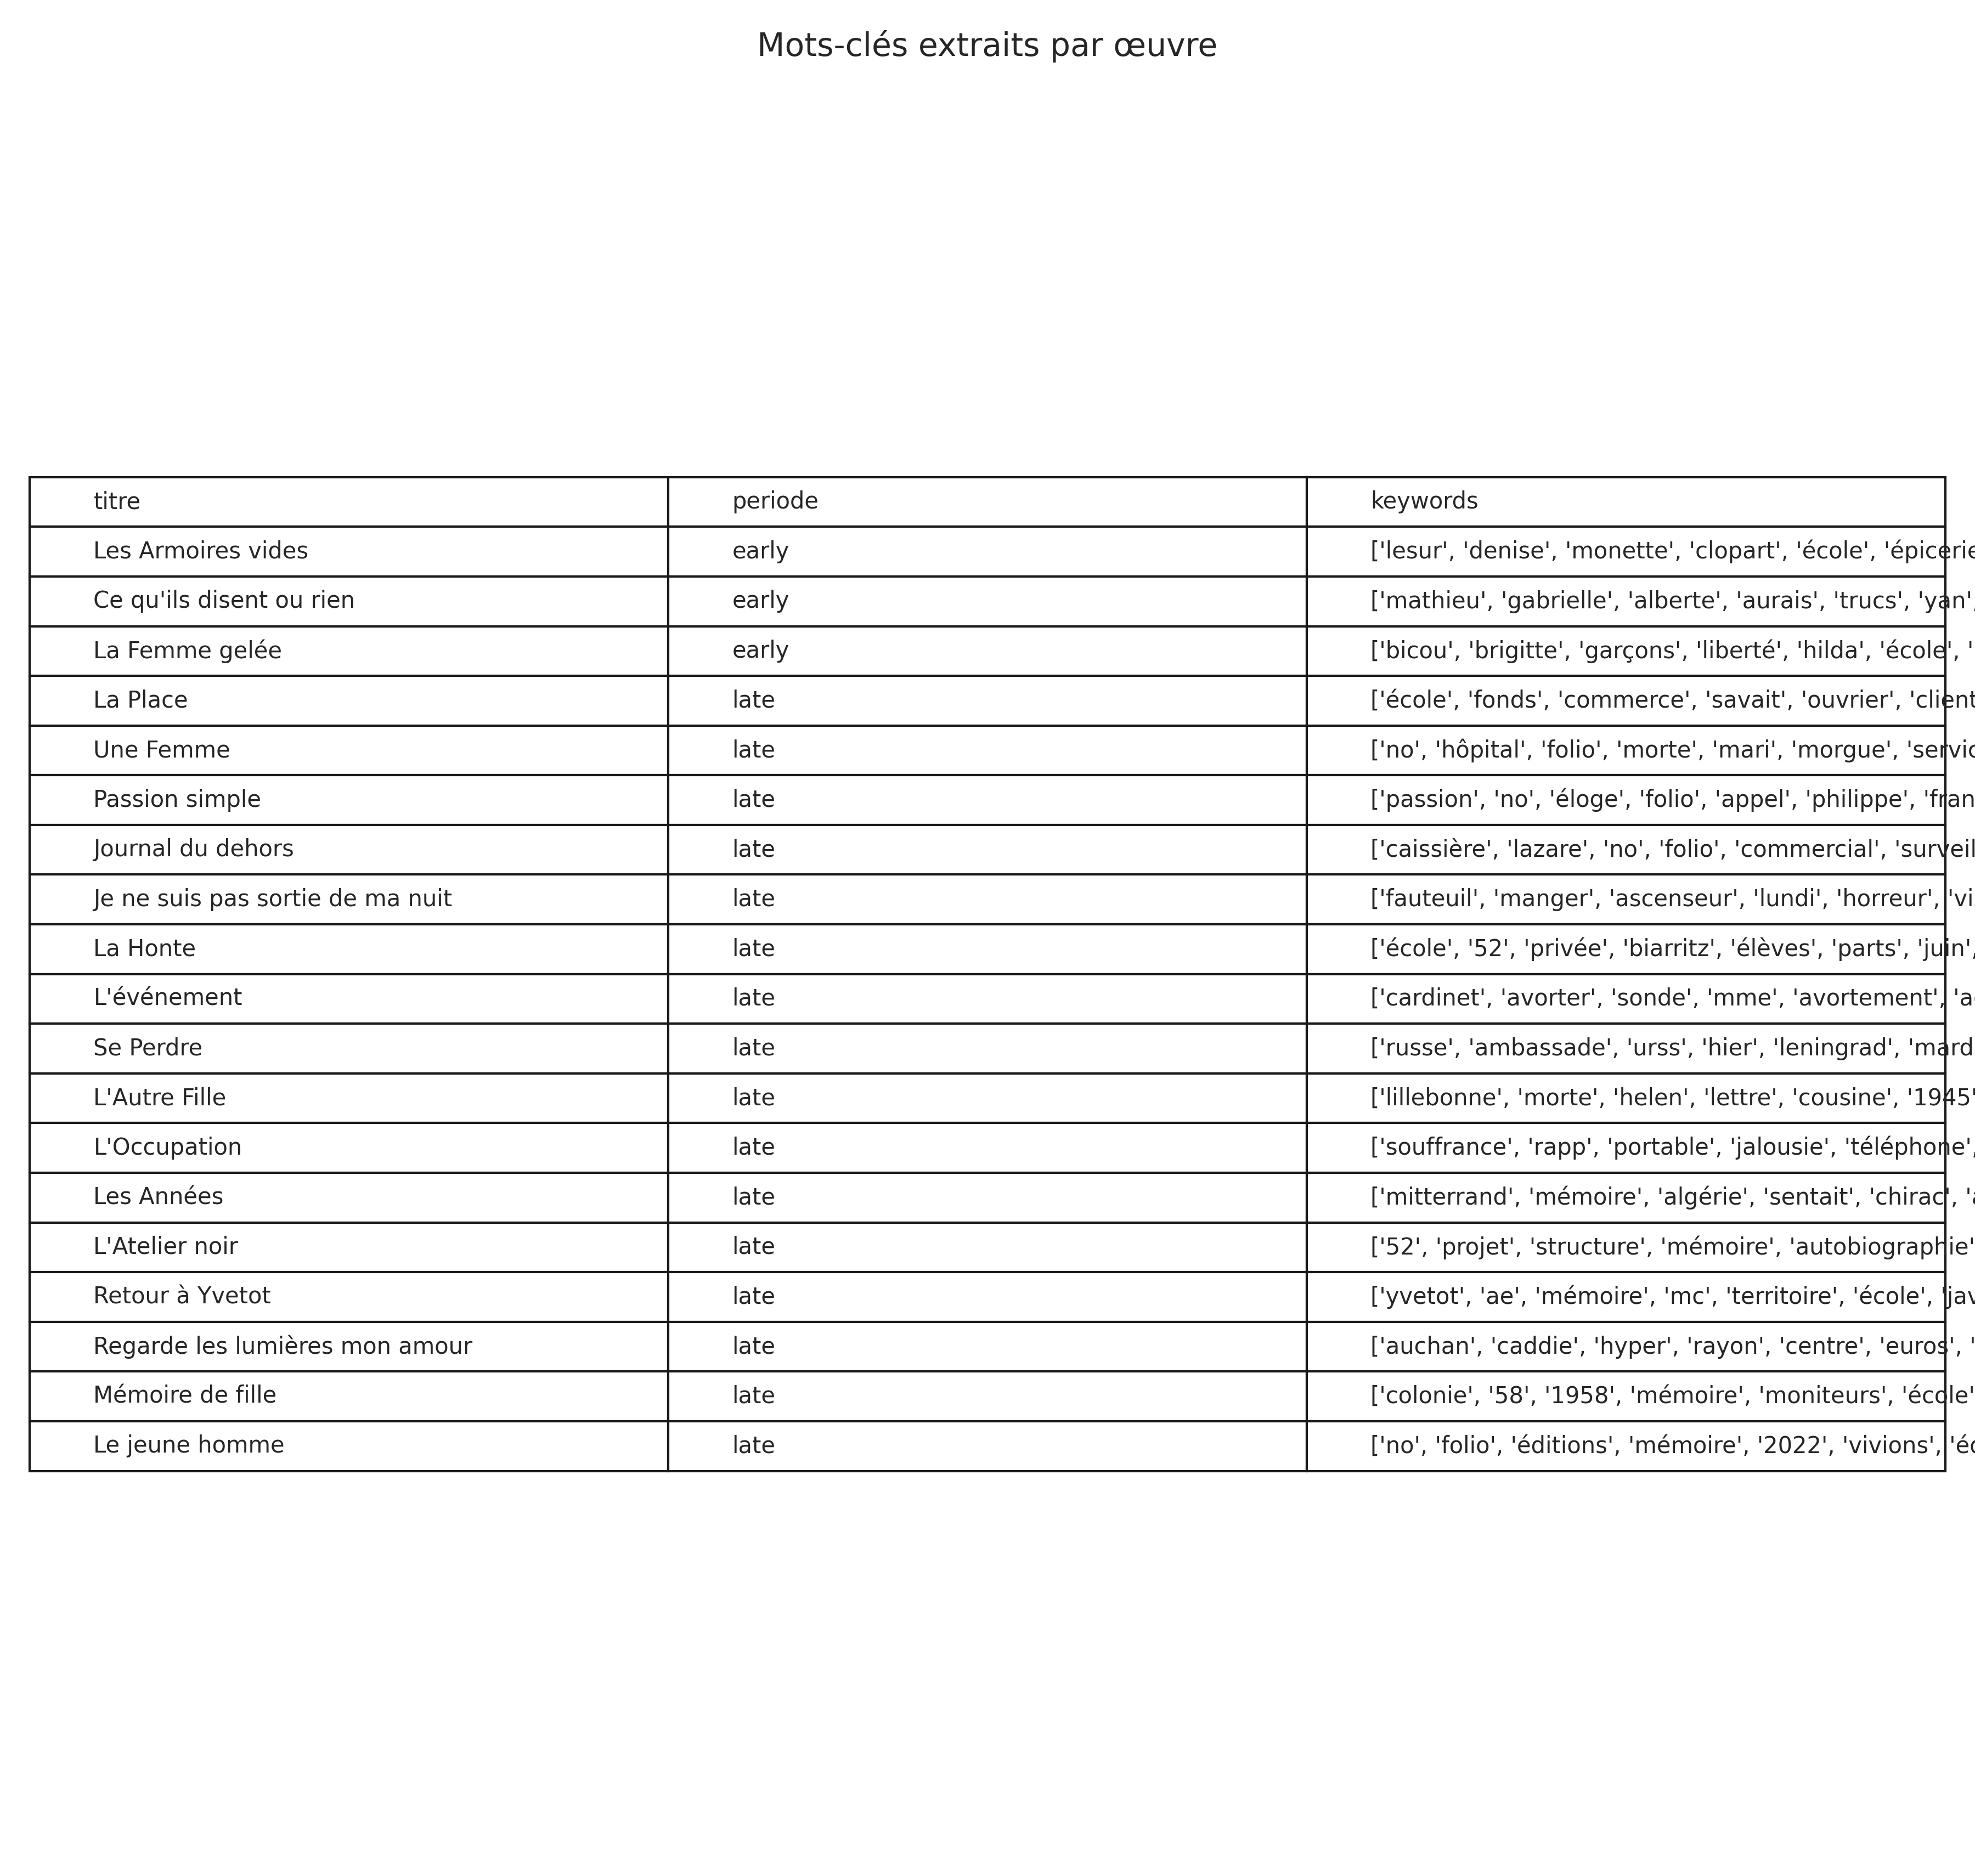
\includegraphics[width=\textwidth]{image/Table_keywords_ernaux.png} % Réduit l'image à 50% de la largeur
        \caption{Liste des mots clés}
        \label{fig:Table de mot-clés des ouvrages d'Ernaux}
    \end{minipage}%
    \hfill
    % Deuxième image à droite
    \begin{minipage}{0.5\textwidth}
        \centering
        \includegraphics[width=\textwidth]{image/Nuages_de_mots_ernaux.png}  % Réduit l'image à 50% de la largeur
        \caption{Nuage de mots}
        \label{fig:Nuage de mots}
    \end{minipage}
\end{figure}

Concernant la classification des thèmes des œuvres, il apparaît que les écrits d'Ernaux se divisent en quatre groupes distincts. Le groupe 0 comprend \textit{Ce qu’ils disent ou rien}, \textit{Je ne suis pas sortie de ma nuit}, \textit{Se Perdre}, \textit{L’Autre Fille}, \textit{L’Occupation} et \textit{Regarde les lumières mon amour}, ces œuvres étant centrées sur des états psychologiques, la solitude, la perte, l’observation et des expériences sociales marginales. Elles présentent une introspection évidente et une écriture spatialement orientée, abordant les frontières sociales telles que la mémoire, l’identité et l’espace urbain. Le groupe 1 inclut \textit{Une Femme}, \textit{Passion simple}, \textit{Journal du dehors}, \textit{L’Événement}, \textit{Les Années}, \textit{L’Atelier noir} et \textit{Le jeune homme}. Ces écrits examinent les expériences féminines et la politique du corps, abordant des thèmes comme l'avortement, les relations amoureuses, les relations mère-fille, et la mémoire historique. Le groupe 2 comprend \textit{Les Armoires vides}, \textit{La Femme gelée}, \textit{La Place} et \textit{La Honte}, où les thèmes se concentrent sur les origines sociales, la mémoire familiale d'enfance et la répression éducative. Le groupe 3 comprend \textit{Retour à Yvetot} et \textit{Mémoire de fille}, qui examinent l'identité régionale, les souvenirs de l’adolescence et le processus de recherche de soi. À travers cette classification, on peut constater que les œuvres d'Ernaux, initialement axées sur des préoccupations familiales et de classe, s’orientent progressivement vers une écriture de mémoire socialisée et historisée, mettant en évidence une évolution profonde de ses thèmes et de son expression personnelle.\\
\begin{figure}[ht!]
    \centering
    \includegraphics[width=\textwidth]{image/Clustering des thèmes de mots-clés de chaque œuvre d'Ernaux.png}
    \caption{Catégorisation thématique}
    \label{fig:Catégorisation thematique}
\end{figure}

 

En ce qui concerne la répartition des temps verbaux, les œuvres d'Ernaux présentent des caractéristiques temporelles distinctes. Le présent de l'indicatif (Indicatif Présent Simple) domine à la fois dans les premiers et derniers travaux, et surtout dans les œuvres récentes, le présent étant davantage utilisé, ce qui correspond à son style d'"autobiographie immédiate" (autobiographie au présent) et renforce le sentiment de présence dans ses écrits. Le passé simple (Passé Simple) est fréquemment employé dans les premières œuvres, utilisé pour les récits linéaires du passé, mais il est progressivement remplacé par le passé composé (Passé Composé) dans les œuvres plus récentes. Le subjonctif présent (Subjonctif Présent Simple) et le conditionnel présent (Conditionnel Présent Simple) sont davantage présents dans les œuvres récentes, notamment dans les explorations des possibilités historiques et des vérités de la mémoire, ce qui témoigne de la réflexion et du doute croissants dans ses écrits. Le présent de l’impératif est pratiquement absent, ce qui reflète le caractère non-directif de son écriture autobiographique.\\
 Répartition des temps verbaux
\begin{figure}[ht!]
    \centering
    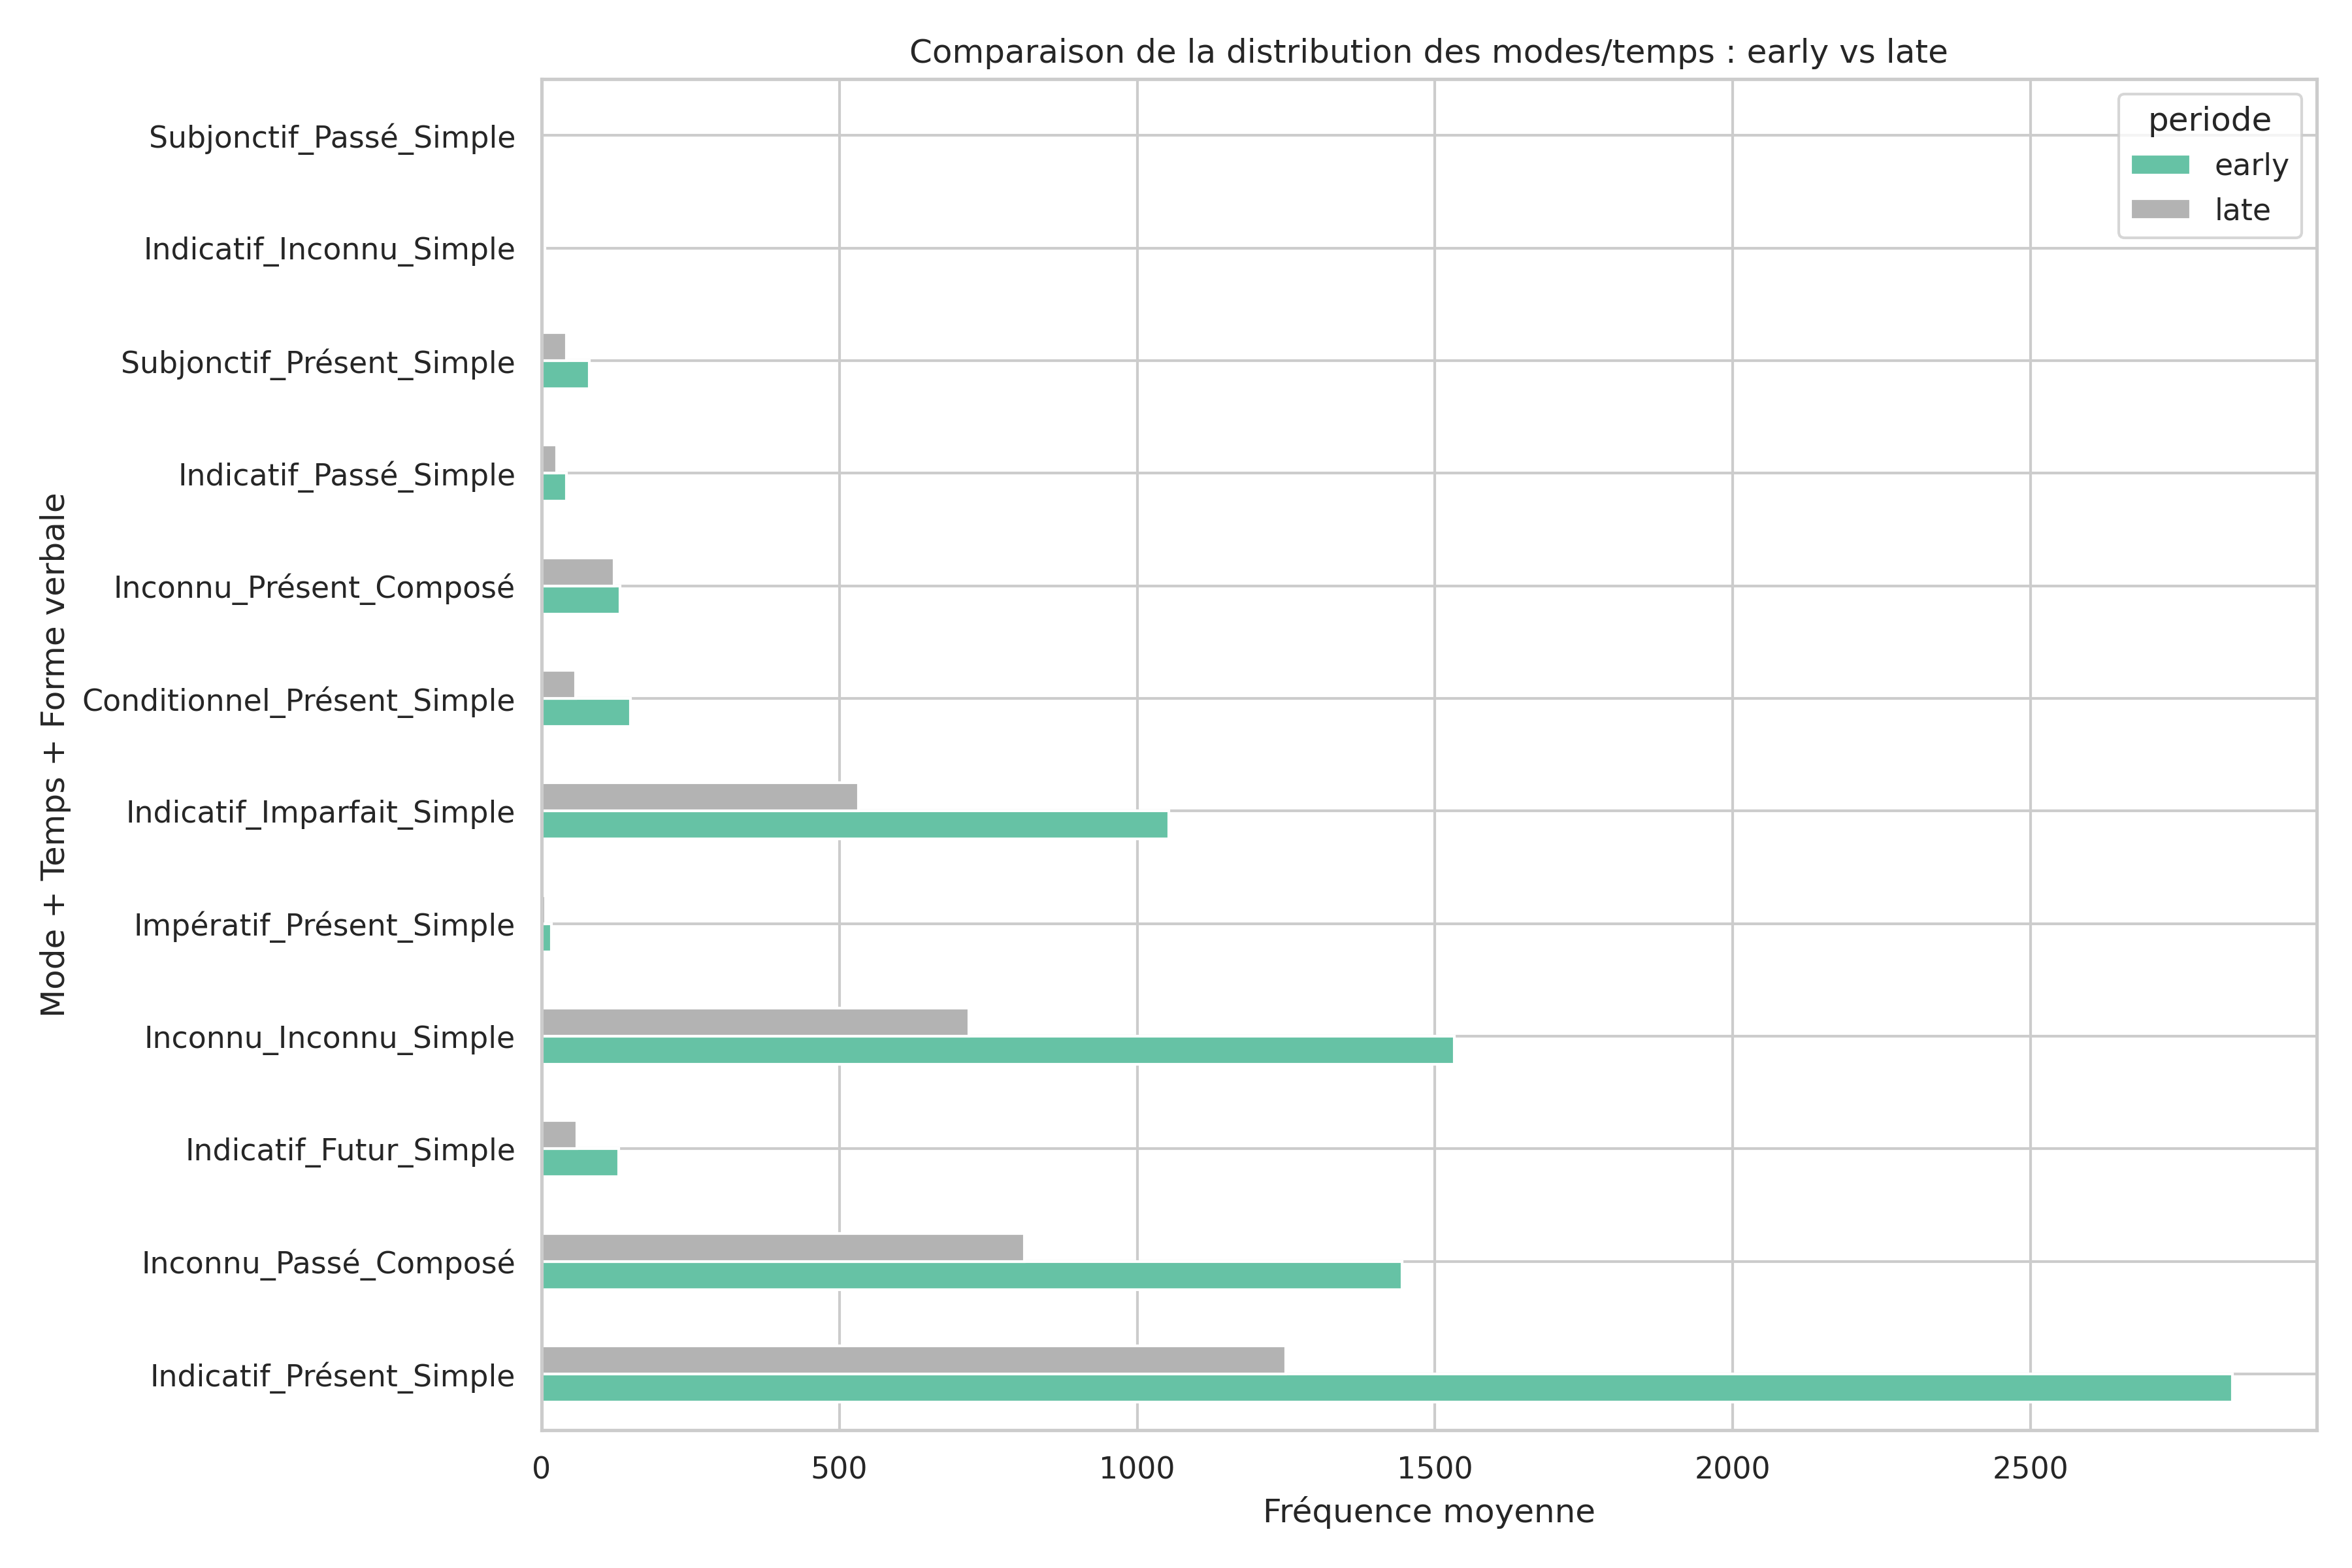
\includegraphics[width=\textwidth]{image/Comparaison_de_la_distribution_des_modes_temps_early_vs_late.png}
    \caption{Répartition des temps verbaux}
    \label{fig:temps verbaux}
\end{figure}

La distribution des pronoms reflète également l’évolution stylistique de l’œuvre d'Ernaux. Le pronom de la première personne "je" domine dans toutes ses œuvres, tant dans les premiers que dans les derniers écrits, avec une légère augmentation dans les œuvres récentes, indiquant un approfondissement de son introspection. Les pronoms de la troisième personne "il" et "elle" deviennent plus fréquents dans ses œuvres tardives, ce qui suggère qu’elle commence à davantage décrire autrui et à réfléchir sur les relations avec les proches ou les "autres" dans la société. L’utilisation du pronom collectif "nous" augmente également dans les œuvres récentes, notamment dans \textit{Les Années}, ce qui illustre l’écriture de la mémoire collective et de l'expérience sociale partagée. Globalement, ses écrits plus tardifs accordent une plus grande attention aux expériences collectives, à la mémoire partagée et aux interactions extérieures, ce qui montre une évolution vers une écriture socialisée et historisée.\\
% Répartition des pronoms
\begin{figure}[ht!]
    \centering
    \includegraphics[width=\textwidth]{image/Fréquence moyenne des pronoms _ early vs late.png}
    \caption{Répartition des pronoms}
    \label{fig:repartition_pronom}
\end{figure}

\newpage

Concernant la distribution du nombre moyen de mots, dans le graphique à barres, nous pouvons observer que certaines œuvres ``récentes'' ont une moyenne de mots par phrase supérieure à celle des œuvres plus anciennes. Par exemple, les phrases dans des œuvres comme \textit{Les Années}, \textit{Ce qu'ils disent ou rien} et \textit{Retour à Yvetot} sont plus longues, ce qui reflète une plus grande complexité. En revanche, certaines œuvres récentes, comme \textit{Passion simple} et \textit{Je ne suis pas sortie de ma nuit}, ont des phrases plus courtes, mettant en avant un style d'écriture plus concis et direct. De manière générale, les œuvres récentes montrent une tendance à la ``diversification'' : certaines adoptent un style minimaliste, tandis que d'autres utilisent des phrases plus longues. Cela indique que la structure des phrases dans les œuvres récentes est devenue plus flexible et variée, reflétant ainsi la diversité du style d'écriture de l'auteure. \\

Dans le diagramme en boîte, nous pouvons observer que les œuvres anciennes (boîte verte) ont une longueur de phrase relativement stable, avec des variations faibles, et une longueur de phrase comprise entre 16 et 25 mots. Cela montre une certaine stabilité et cohérence. En revanche, les œuvres récentes (boîte orange) montrent une plus grande variation, avec des longueurs de phrase allant de 10 à près de 25 mots, indiquant davantage de fluctuation et d'incertitude. Cependant, la plupart des phrases dans les œuvres récentes ont un nombre moyen de mots inférieur à 20, et surtout, dans \textit{Passion simple}, un point bas est observable avec une moyenne de seulement 10,53 mots. La médiane des œuvres récentes est inférieure à celle des œuvres anciennes, ce qui suggère que l'auteure tend à utiliser des phrases plus courtes, probablement pour accentuer la simplicité et la directivité de son langage. Toutefois, la plus grande variation dans les œuvres récentes montre également une complexité accrue du style, témoignant d'une utilisation plus libre et plus diversifiée des structures de phrases.\\
\begin{figure}[ht!]
    \centering
    \begin{subfigure}[b]{0.8\textwidth}
        \centering
        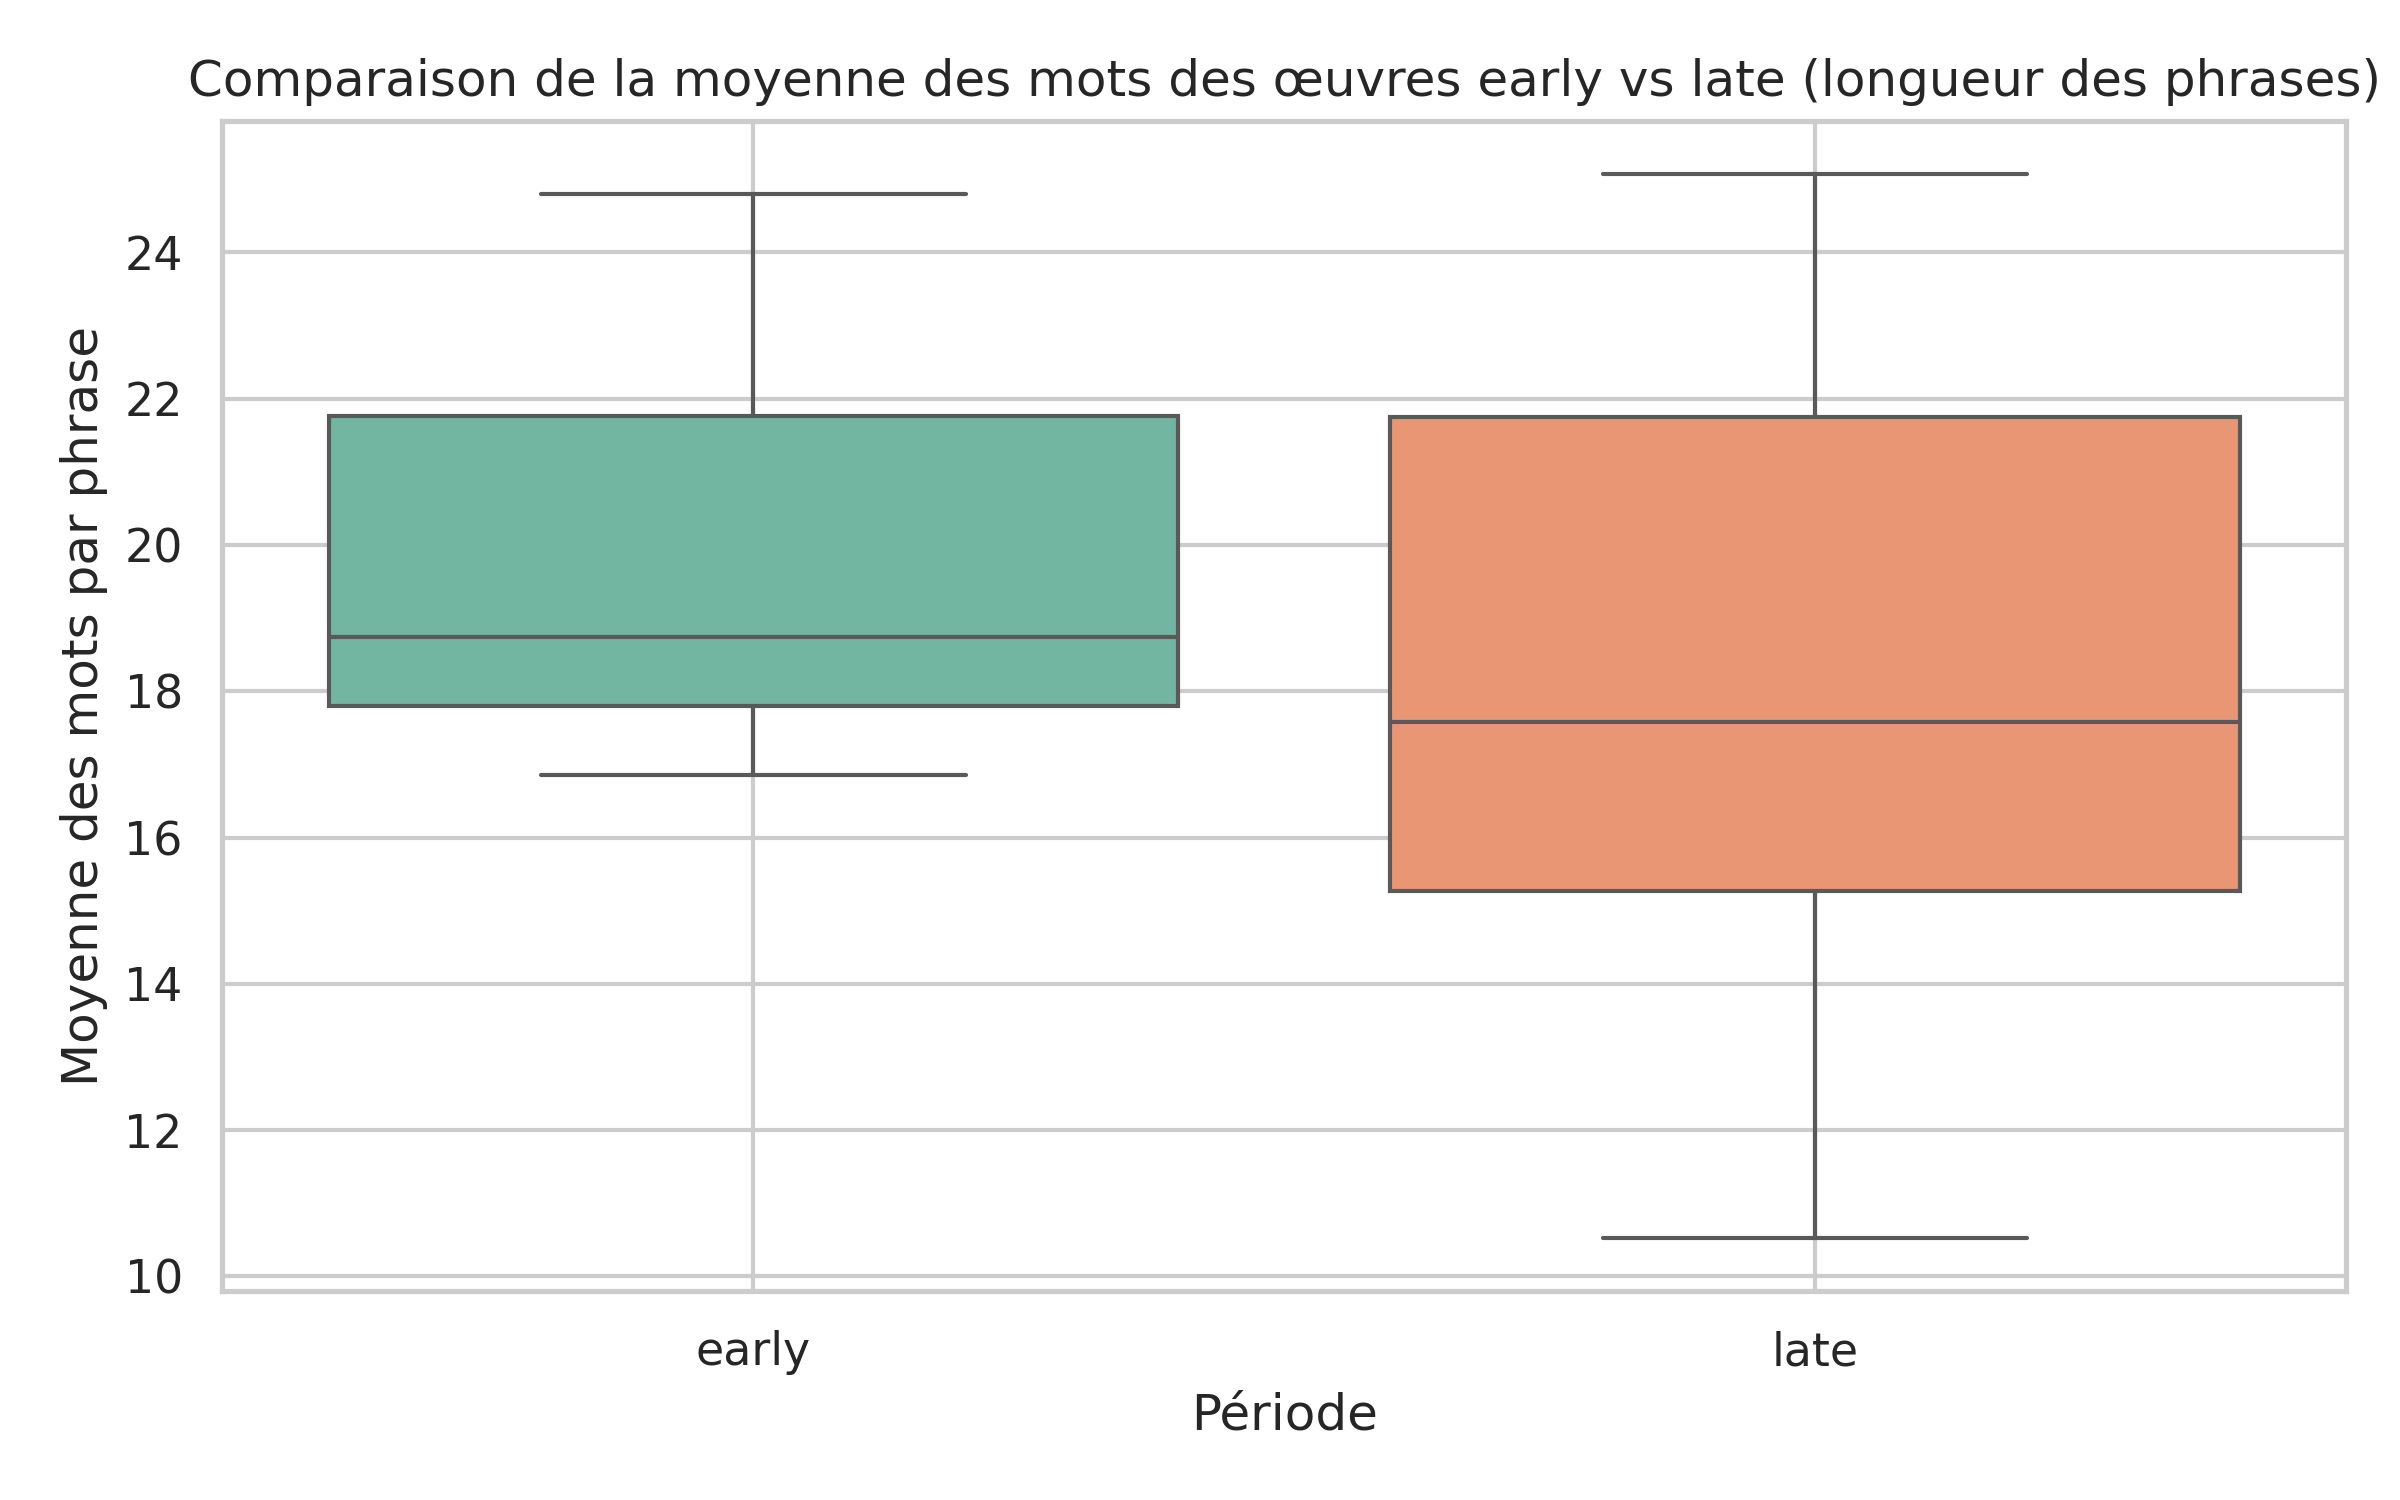
\includegraphics[width=\textwidth]{image/Comparaison de la moyenne des mots des galactiches early vs late (longueur des phrases).png}
        \caption{Répartition des mots moyens (graphique 1)}
        \label{fig:mots_moyens_boite}
    \end{subfigure}
    \vspace{1em} % Espace entre les deux images
    \begin{subfigure}[b]{0.8\textwidth}
        \centering
        \includegraphics[width=\textwidth]{image/Longueur moyenne des phrases de chaque œuvre (par nombre de mots).png}
        \caption{Répartition des mots moyens (graphique 2)}
        \label{fig:mots_moyens_barres}
    \end{subfigure}
    \caption{Comparaison des répartitions des mots moyens entre les œuvres}
    \label{fig:mots_moyens_comparison}
\end{figure}
\newpage
Concernant le TTR (Type-Token Ratio), dans la comparaison des diagrammes en boîte du TTR, la médiane du TTR des œuvres tardives est d'environ 0,48, bien plus élevée que celle des œuvres précoces (environ 0,36). Cette différence indique que les œuvres tardives présentent une plus grande diversité et richesse lexicale. La valeur maximale du TTR des œuvres tardives dépasse largement celle des œuvres précoces, et on observe une plus grande variabilité des textes, ce qui montre que l'auteur adopte une utilisation lexicale plus diversifiée dans ses créations ultérieures. Toutefois, certaines œuvres tardives, comme \textit{Ce qu'ils disent ou rien}, présentent un TTR relativement faible, ce qui suggère que toutes les œuvres tardives ne montrent pas une expansion lexicale significative. En réalité, les œuvres tardives ne sont pas pauvres en vocabulaire, mais elles adoptent une stratégie linguistique plus personnalisée : certaines œuvres utilisent un vocabulaire minimal, tandis que d'autres exhibent une grande variété lexicale.\\

Dans le diagramme en barres du TTR, nous pouvons observer que l'œuvre ayant le TTR le plus élevé parmi les œuvres tardives est \textit{Le jeune homme}, avec un TTR d'environ 0,69, ce qui démontre une utilisation très variée du vocabulaire. En revanche, les œuvres avec une faible richesse lexicale incluent \textit{Se Perdre}, ainsi que les œuvres précoces comme \textit{Les Armoires vides} et \textit{Ce qu'ils disent ou rien}, qui présentent un taux de répétition lexical élevé et traduisent un style d'écriture plus concis. Il est donc clair que toutes les œuvres tardives ne suivent pas la tendance de "simplification" ou de "minimalisme". En fait, l'auteur choisit parfois délibérément d’utiliser un langage plus succinct et répétitif, créant ainsi des contextes et des atmosphères différentes. Par conséquent, les œuvres tardives révèlent une multiplicité de possibilités en termes d’utilisation du vocabulaire : parfois un style minimaliste, parfois une grande fréquence de variation lexicale, ce qui reflète l’exploration plus flexible et diversifiée du langage par l’auteure. En somme, les œuvres précoces et tardives montrent des différences notables dans l'utilisation du vocabulaire et la longueur des phrases, les œuvres tardives présentant un style d’écriture plus riche et diversifié, tout en manifestant une utilisation linguistique plus individualisée, qui reflète différentes stratégies et formes d’expression linguistique.

% Répartition du TTR
\begin{figure}[ht!]
    \centering
    \includegraphics[width=\textwidth]{image/Comparaison de la richesse lexicale des œuvres early et late (TTR).png}
    \caption{Répartition du TTR}
    \label{fig:repartition_TTR_boite}
\end{figure} 
\begin{figure}[ht!]
    \centering
    \includegraphics[width=\textwidth]{image/Répartition de la richesse lexicale des œuvres (TTR).png}
    \caption{Répartition du TTR}
    \label{fig:repartition_TTR_barres}
\end{figure} 

\newpage

\subsection{Analyse syntaxique}
Les structures des phrases dans les premiers et derniers travaux d'Ernaux diffèrent de manière marquée. Dans les premières œuvres, la longueur moyenne des phrases reste relativement stable, généralement entre 16 et 25 mots, tandis que dans les œuvres récentes, la longueur des phrases varie davantage, surtout dans \textit{Passion simple} et \textit{Je ne suis pas sortie de ma nuit}, où l’on observe des phrases plus courtes. Les œuvres récentes tendent vers une syntaxe plus concise, bien qu’il y ait également des phrases plus longues, reflétant une diversification de son style. De plus, la richesse lexicale (TTR) augmente de manière significative dans les œuvres récentes, ce qui témoigne d’une utilisation plus variée du vocabulaire. Bien que certaines œuvres récentes comme \textit{Ce qu’ils disent ou rien} présentent un TTR plus bas, elles présentent globalement une stratégie linguistique plus individualisée.\\
% Catégories grammaticales 
\begin{figure}[ht!]
    \centering
    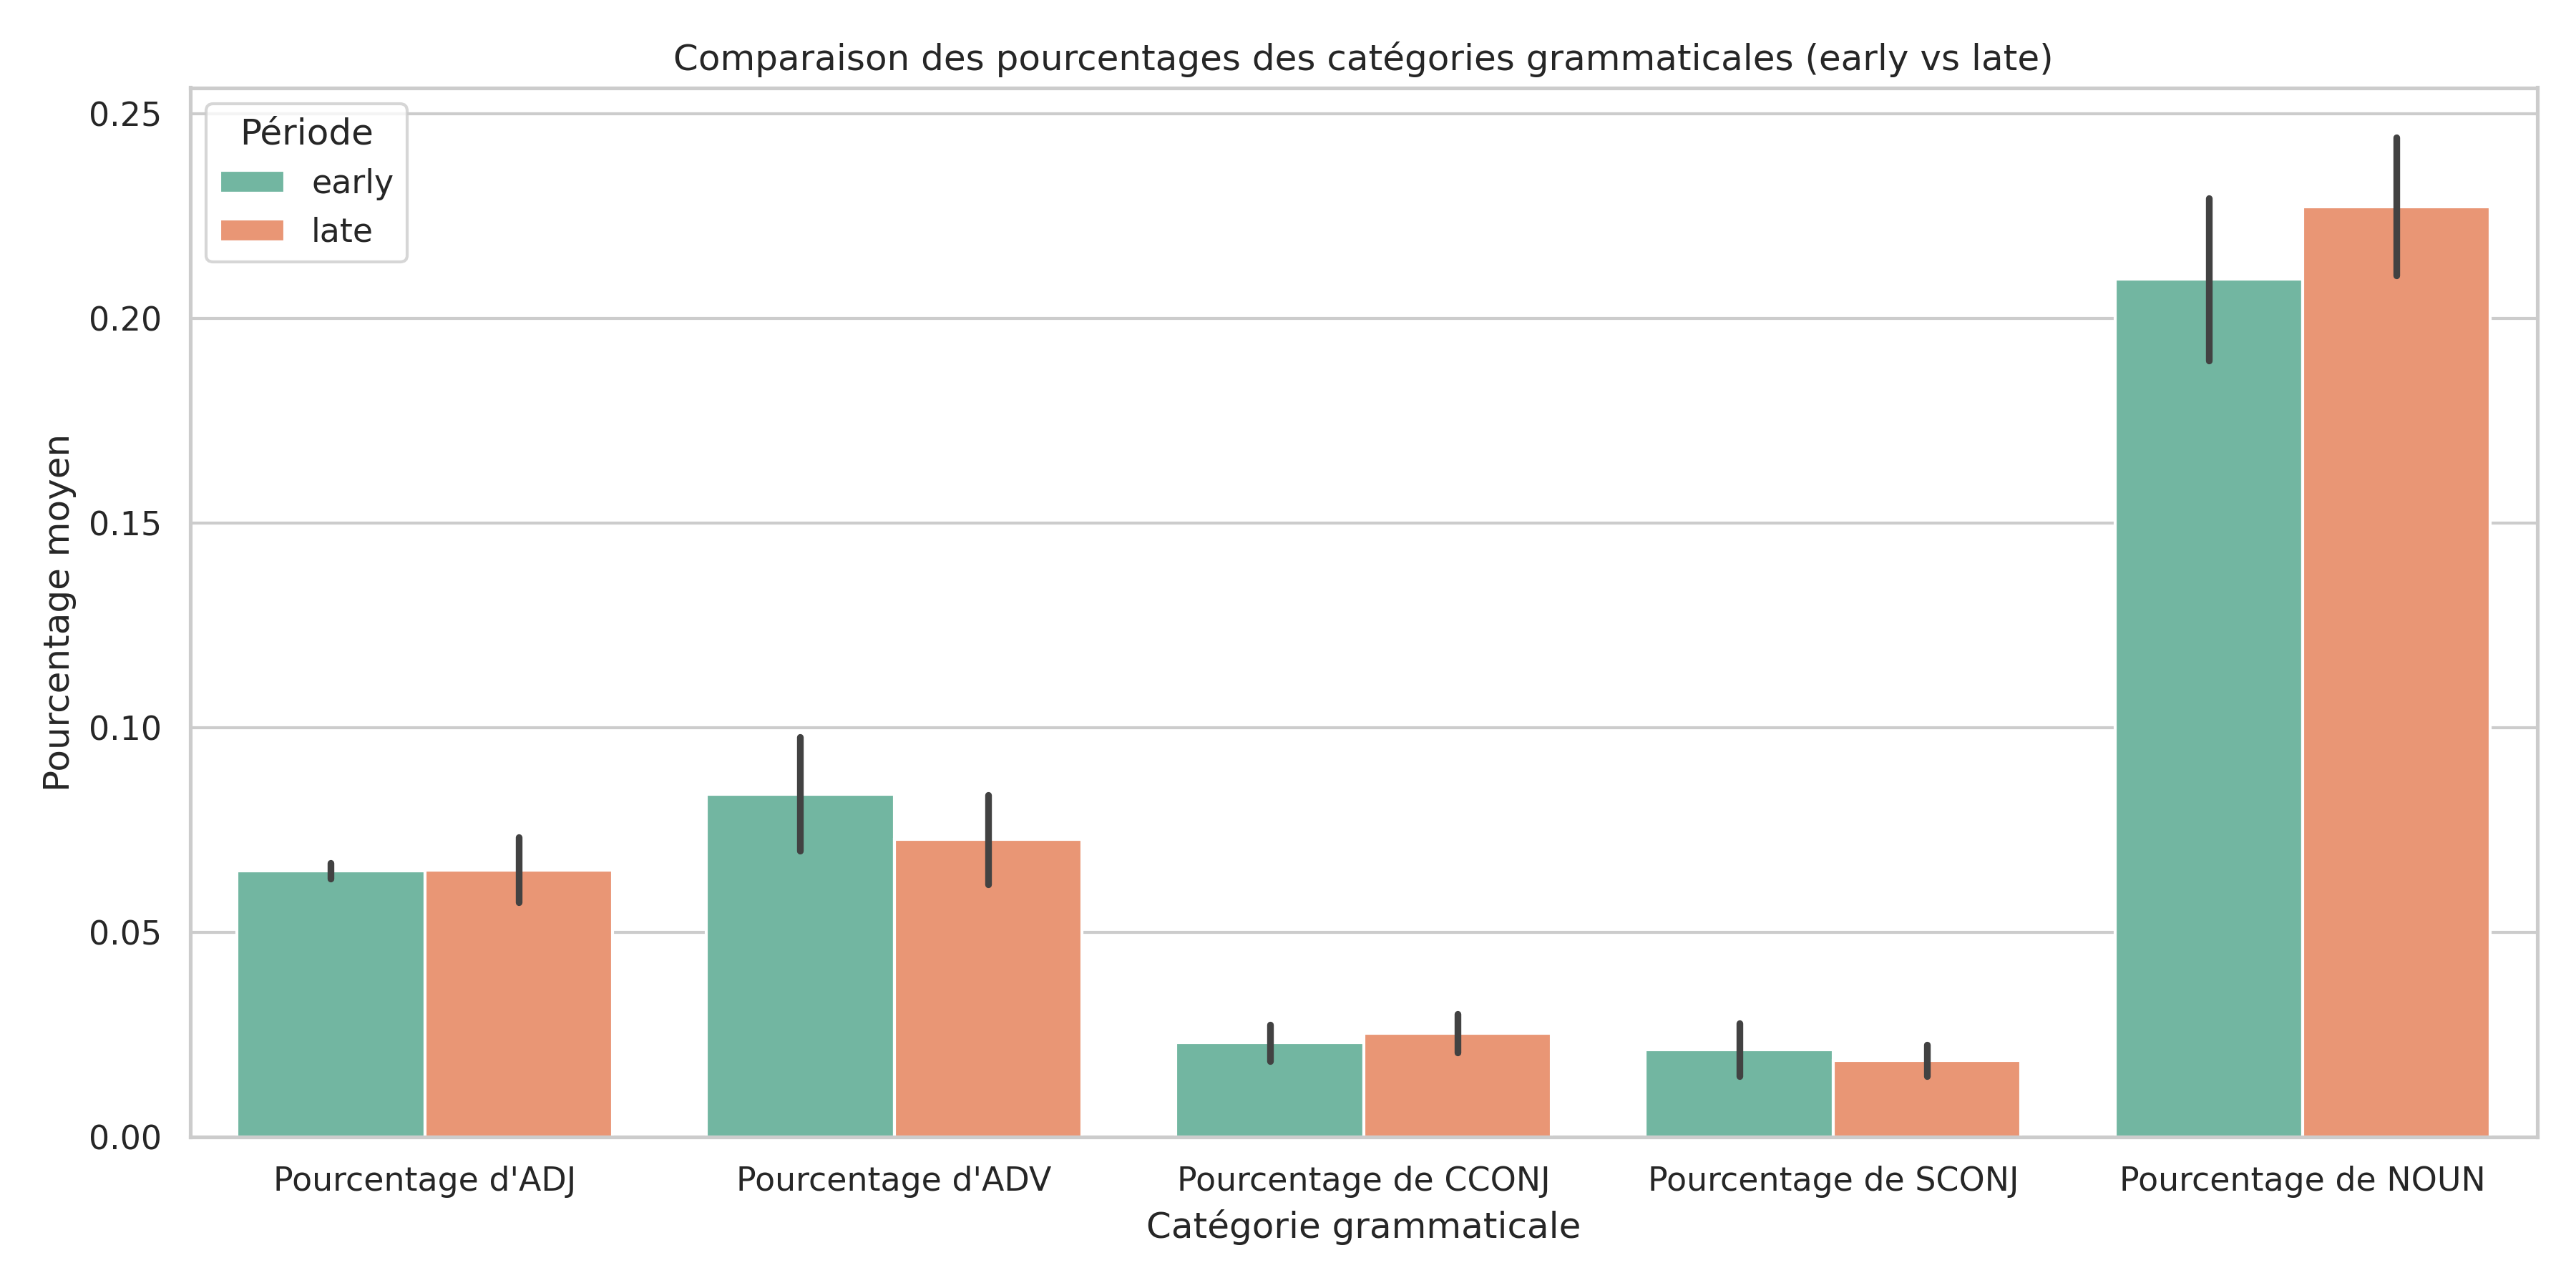
\includegraphics[width=\textwidth]{image/Comparaison des pourcentages des catégories grammaticales (early vs late).png}
    \caption{Répartition des catégories grammaticales}
    \label{fig:catégories grammaticales}
\end{figure}

\newpage

\subsection{Analyse rhétorique}
Les œuvres d'Ernaux présentent une utilisation relativement sobre de la répétition. La plupart de ses textes montrent une faible densité de répétition, en particulier dans les œuvres non-diatétiques. Cependant, dans \textit{Je ne suis pas sortie de ma nuit}, en raison de son format de journal, la répétition est plus présente et contribue à une intensification expressive. L'utilisation des parallélismes est assez rare et se retrouve principalement dans les œuvres plus récentes comme \textit{Une femme} et \textit{Passion simple}, où les structures parallèles et les phrases structurées renforcent le rythme et l’intensité de l’écriture.\\

D'après ces analyses, les indicateurs quantitatifs du "style simple" sont définis par une moyenne de TTR de 0.4 et une longueur moyenne de phrase de 18 mots. Les œuvres d'Ernaux, avec leurs caractéristiques en termes de TTR et de longueur des phrases, répondent aux critères du style simple, en particulier dans ses premiers écrits où le TTR est plus bas, tandis que les œuvres récentes montrent une réduction de la longueur des phrases, ce qui témoigne d'un style d'écriture plus concis.
% Répartition des répétitions
\begin{figure}[ht!]
    \centering
    \includegraphics[width=\textwidth]{image/Densité de repetition_density par œuvre.png}
    \caption{Répartition des répétitions}
    \label{fig:repartition_repetitions}
\end{figure}

\vspace{1cm}

% Répartition des parallélismes
\begin{figure}[ht!]
    \centering
    \includegraphics[width=\textwidth]{image/Densité de parallelism_density par œuvre.png}
    \caption{Répartition des parallélismes}
    \label{fig:repartition_parallels}
\end{figure}

\newpage

\section{Corpus externe}
Dans le corpus externe, l’analyse du TTR et de la longueur moyenne des phrases d’autres écrivains montre des similitudes et des différences avec le style d'Ernaux. Par exemple, le TTR de Yourcenar varie entre 0.45 et 0.5, avec des phrases généralement plus longues (plus de 20 mots), ce qui reflète un style plus complexe et élégant ; celui de Robbe-Grillet est plus bas (environ 0.35), avec des phrases plus courtes (entre 15 et 18 mots), représentant son style de description précis et minimaliste caractéristique du "nouveau roman" ; le TTR de Sartre est plus élevé (environ 0.5), et ses phrases sont plus longues, ce qui reflète une structure complexe et un texte à forte dimension philosophique ; Simon a un TTR élevé et des phrases relativement courtes, caractérisant un style sobre ; enfin, Pinget et Green présentent un TTR bas avec des phrases courtes, ce qui témoigne d’un style simple et direct.\\

Comparé à ces écrivains, le style d'Ernaux se situe dans le cadre de l’écriture "simple". En effet, le TTR d'Ernaux est relativement bas, et la longueur de ses phrases est courte, ce qui le rapproche du style de Robbe-Grillet. Toutefois, son écriture se distingue par une dimension sociologique et historique plus marquée. Elle utilise un vocabulaire précis pour analyser les classes sociales et décrire des expériences corporelles, ce qui crée une autobiographie distinctive. Parmi les écrivains du corpus externe, le style d'Ernaux se distingue, particulièrement dans l’utilisation du vocabulaire, et même si son TTR est légèrement plus élevé que celui de Robbe-Grillet, il demeure plus simple et direct que celui de Sartre, tout en mettant l’accent sur le contexte social et historique.
\begin{figure}[ht!]
    \centering
    \begin{subfigure}[b]{0.8\textwidth}
        \centering
        \includegraphics[width=\textwidth]{image/TTR par œuvre (corpus externe).png}
        \caption{Répartition du TTR pour chaque œuvre}
        \label{fig:TTR_externe}
    \end{subfigure}
    
    \vspace{0.5cm} % Ajouter un peu d'espace entre les deux images

    \begin{subfigure}[b]{0.8\textwidth}
        \centering
        \includegraphics[width=\textwidth]{image/Longueur moyenne des phrases par œuvre (corpus externe).png}
        \caption{Répartition du nombre moyen de mots pour chaque œuvre}
        \label{fig:mots_moyens_externe}
    \end{subfigure}
\end{figure}

